\chapter{Mediciones y resultados}
En este capítulo se presentan los resultados del diseño del protocolo SPI utilizado para controlar los convertidores D/A y A/D, así como los resultados obtenidos de la caracterización de resistencias, multiplexores y fotorresistencia. Además, se muestran las imágenes generadas por la matriz de fototransistores, evidenciando el correcto funcionamiento del sistema de adquisición de datos implementado y de la PCB diseñada.


\section{Resultados de protocolo SPI}
Para probar el funcionamiento del diseño del protocolo SPI, se utilizó un potenciómetro al que se varió la resistencia, conectado a un canal del convertidor A/D. Para evaluar el convertidor D/A, se asignó un valor de voltaje en formato binario. Las señales generadas por los módulos implementados en la FPGA, junto con las conversiones realizadas por el ADC y DAC, fueron visualizadas mediante un osciloscopio y un multímetro. En esta sección se explicarán los resultados obtenidos de ambos convertidores.

\subsection{ADC}
En el ADC se utilizó el protocolo de lectura y escritura del SPI. De acuerdo al datasheet, una conversión completa requiere 25 ciclos de dclk: durante los primeros 8 ciclos se configura el ADC, luego se deja pasar un ciclo, y en los siguientes 16 ciclos se realiza la conversión. El ADC realiza la conversión en grupos de 8 bits.


En las capturas del osciloscopio (Figura \ref{fig:ss_osc_adc_2v} y Figura \ref{fig:ss_osc_adc_3v}) se visualizan cuatro señales numeradas del 1 al 4. La señal 1 corresponde al comando de configuración del ADC, la señal 2 al reloj dclk, la señal 3 a la conversión realizada por el ADC, y la señal 4 al chip select (CS). Es importante destacar que las señales 1, 2, y 4 son generadas por los módulos diseñados e implementados en la FPGA, mientras que la señal 3 proviene directamente del ADC, mostrando el resultado de la conversión.


Se realizaron dos pruebas para comprobar el funcionamiento del SPI. En la primera se conectó un potenciómetro al canal 0 del ADC y se configuró hasta obtener un voltaje de 2V. En la siguiente figura se puede observar la conexión.

            \begin{figure}[hbtp]
                \centering
                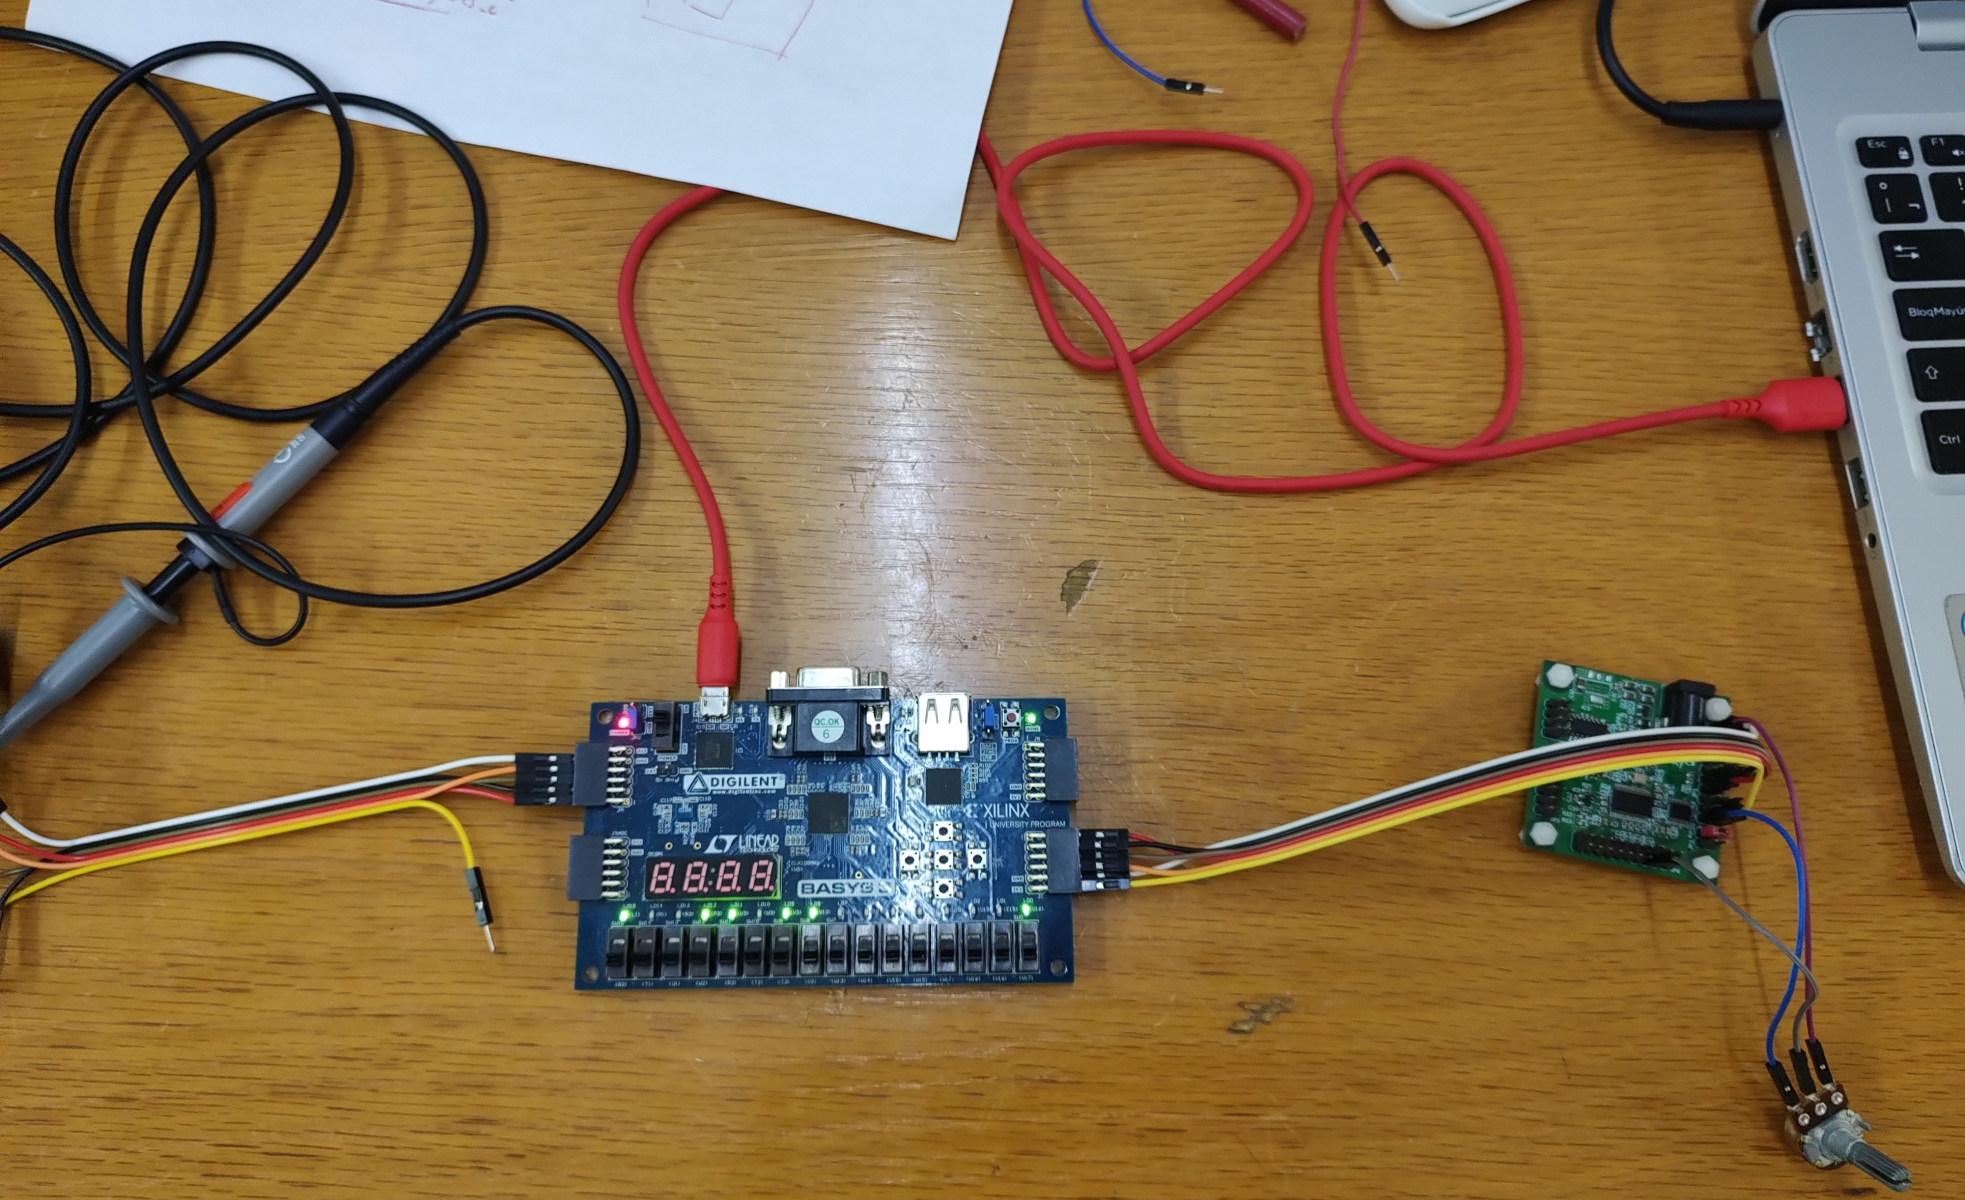
\includegraphics[width=0.6\textwidth]{adc_pot}
                \caption{Arreglo de potenciómetro, ADC y tarjeta Basys 3.}
                \label{fig:adc_pot}
            \end{figure}


 En la Figura \ref{fig:ss_osc_adc_2v} se muestra la conversión realizada por el dispositivo, evidenciando el funcionamiento del diseño del protocolo SPI y del ADC al realizar la conversión de la señal analógica a digital.

            \begin{figure}[hbtp]
                \centering
                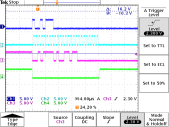
\includegraphics[width=0.6\textwidth]{ss_osc_adc_2v}
                \caption{Captura de osciloscopio de la conversión de 2V realizada por el ADC.}
                \label{fig:ss_osc_adc_2v}
            \end{figure} 

La conversión en el ADC comienza a partir del décimo pulso del dclk. En este caso, la conversión resultante fue 1001 1011 0000, lo que equivale a 2480 en decimal. Realizando una regla de tres, se obtiene que este valor corresponde a un voltaje de 1.9985V.


La segunda prueba consistió en aplicar 3.3V al canal 0 del ADC para evaluar su respuesta ante un voltaje mayor. En la siguiente figura se muestra la conversión resultante
            \begin{figure}[hbtp]
                \centering
                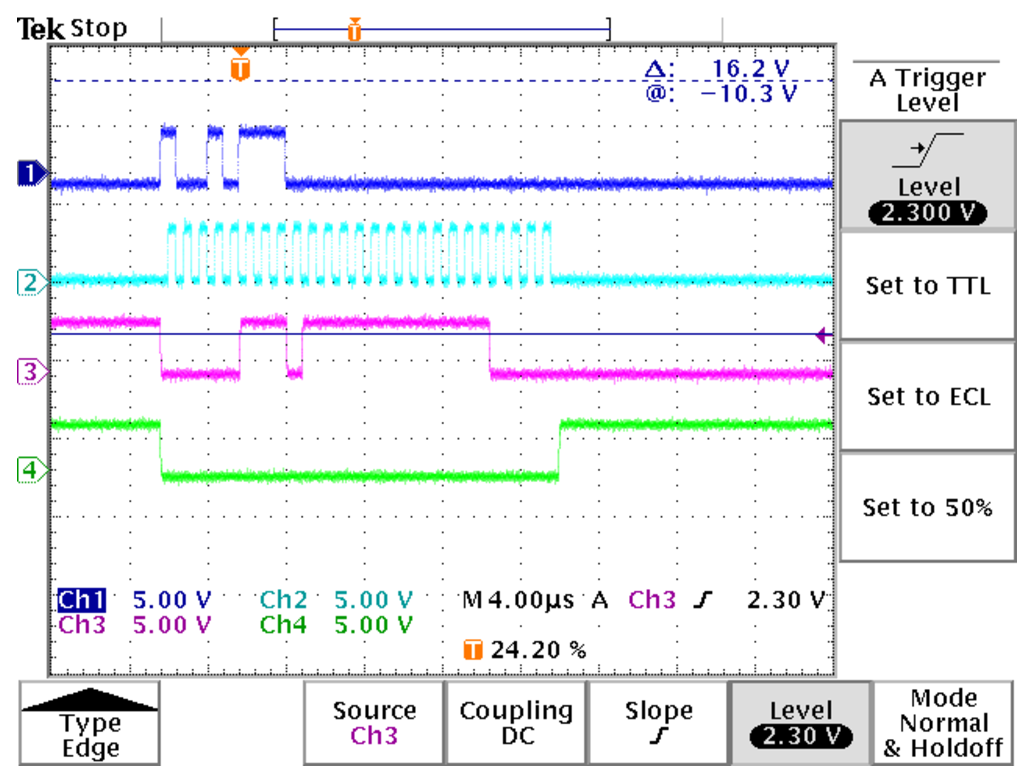
\includegraphics[width=0.6\textwidth]{ss_osc_adc_3v}
                \caption{Captura de osciloscopio de la conversión de 3.3V realizada por el ADC.}
                \label{fig:ss_osc_adc_3v}
            \end{figure} 

El resultado de la conversión fue 1111 1111 1111, que corresponde a 4095 en decimal. Este valor equivale a un voltaje de 3.3V, confirmando que el ADC realizó correctamente la conversión de la señal analógica al valor digital máximo posible para este canal.
     
\subsection{DAC}
Para controlar el DAC, se utilizó únicamente la escritura a través del protocolo SPI. Basándonos en el datasheet del DAC, la escritura se realiza en 16 ciclos de sck. Durante los primeros 4 ciclos, se envía el comando de configuración, en el cual se especifica en qué canal se tendrá el resultado de la conversión. En los 12 ciclos restantes, se transmite un valor de voltaje en formato binario de 12 bits al dispositivo para su conversión a señal analógica.


En las Figuras \ref{fig:ss_osc_dac_2v} y \ref{fig:ss_osc_dac_3v} se muestran las capturas del osciloscopio, donde se pueden observar tres señales numeradas del 1 al 3. La señal número 1 corresponde a los pulsos de reloj sck, la señal número 2 muestra el comando y el valor del voltaje en formato binario, y la señal número 3 representa el chip select del dispositivo. Todas estas señales fueron generadas por los módulos de diseño del protocolo SPI implementado.


Para verificar que el DAC realizara correctamente la conversión, se asignaron dos valores de voltaje en formato binario al MOSI: 1001 1011 0010, equivalente a 2V, y 1111 1111 1111, equivalente a 3.3V. Posteriormente, se midió el voltaje en el canal asignado utilizando un multímetro, confirmando que las conversiones fueron precisas.


En las siguientes imágenes se muestran las capturas del osciloscopio correspondientes a la escritura del DAC, así como el resultado en el multímetro de la conversión de 2V y 3.3V, respectivamente.

            \begin{figure}[hbtp]
                \centering
                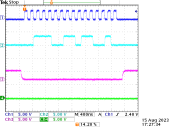
\includegraphics[width=0.6\textwidth]{ss_osc_dac_2v}
                \caption{Captura de osciloscopio de la escritura de 2V en binario en el DAC.}
                \label{fig:ss_osc_dac_2v}
            \end{figure}
            
            \begin{figure}[hbtp]
                \centering
                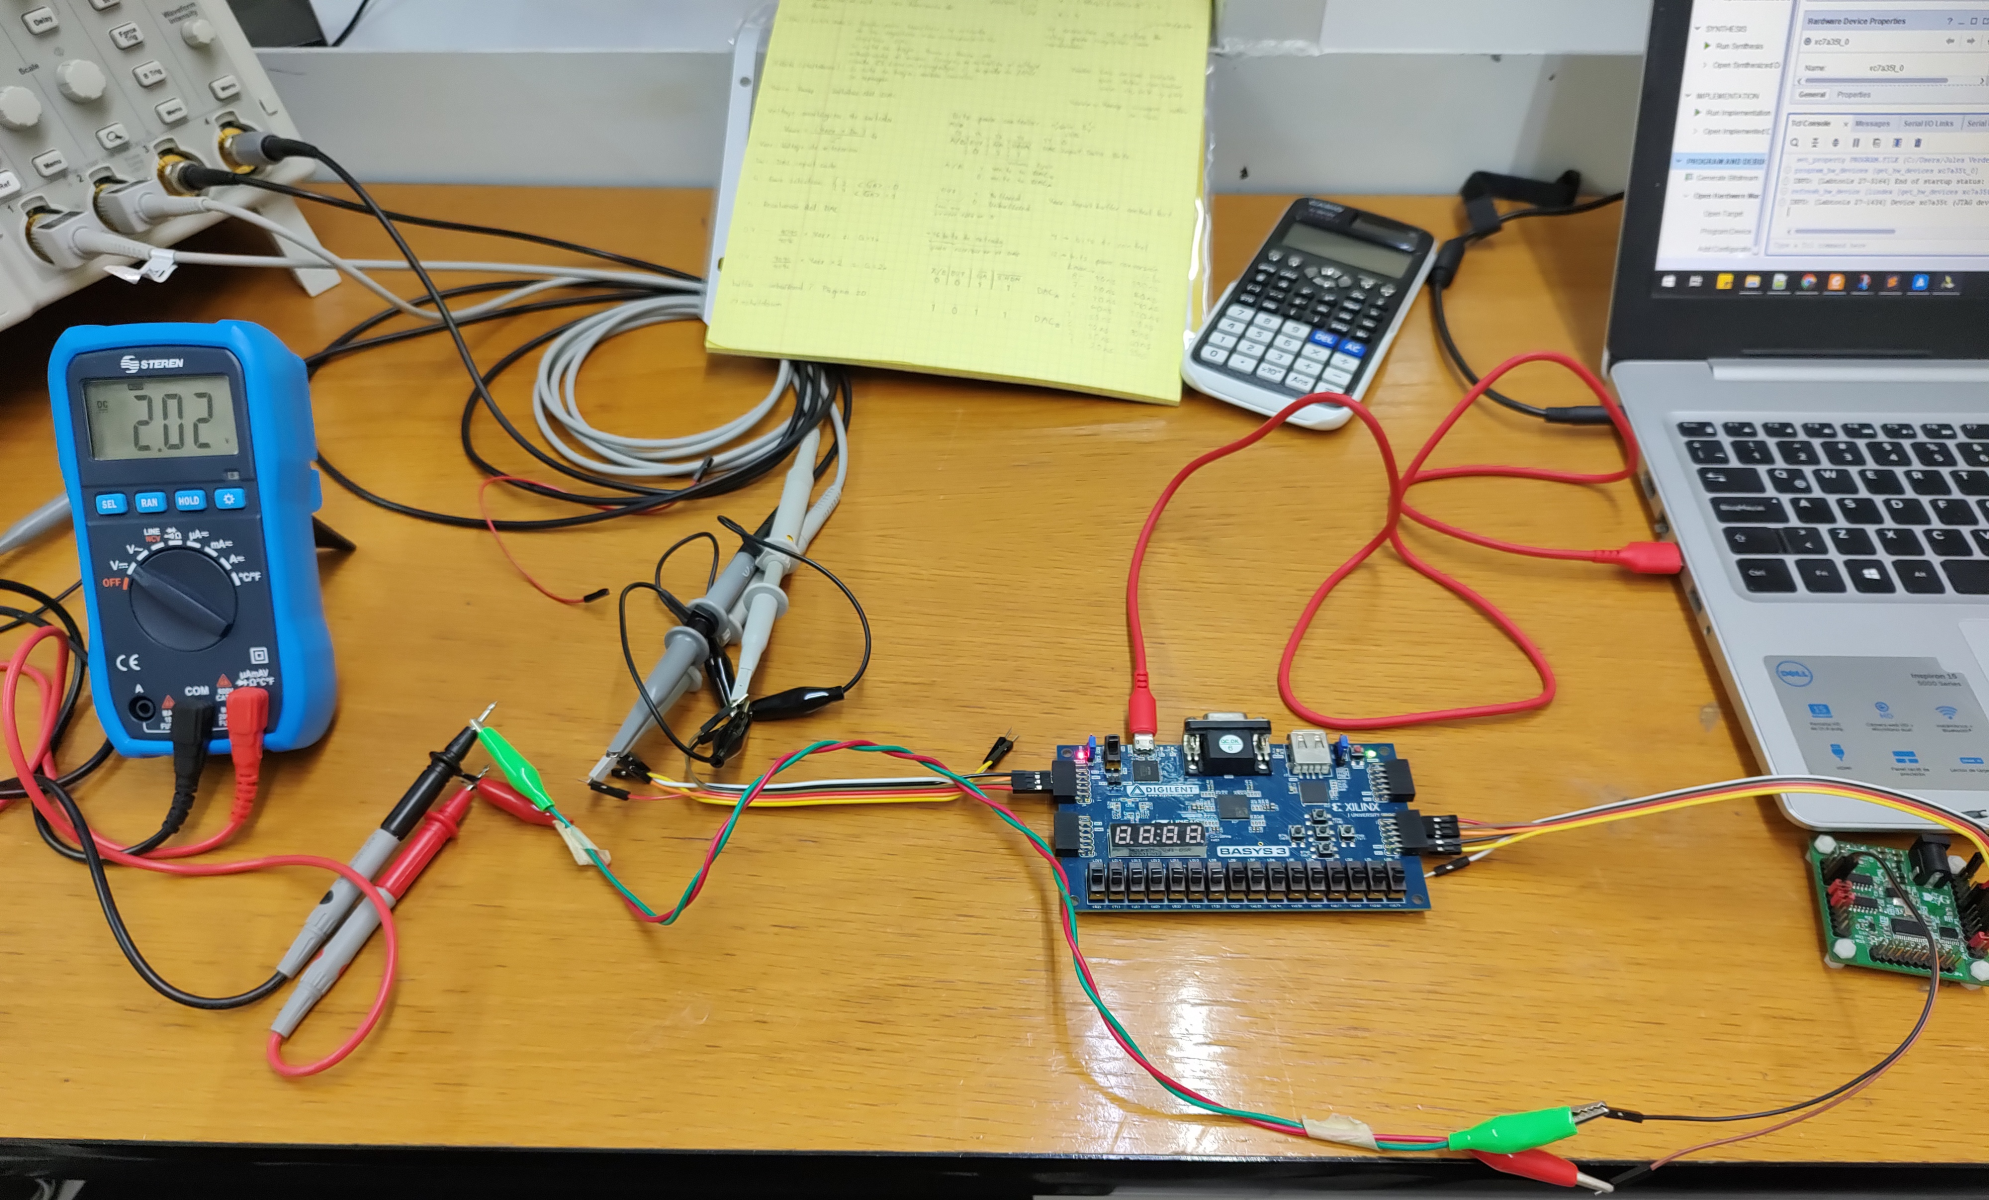
\includegraphics[width=0.6\textwidth]{dac_conversion_2v}
                \caption{Resultado de la conversión de 2V realizada por el DAC.}
                \label{fig:dac_conversion_2v}
            \end{figure}            
          
            \begin{figure}[hbtp]
                \centering
                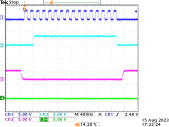
\includegraphics[width=0.6\textwidth]{ss_osc_dac_3v}
                \caption{Captura de osciloscopio de la escritura de 3.3V en binario en el DAC}
                \label{fig:ss_osc_dac_3v}
            \end{figure}   

            \begin{figure}[hbtp]
                \centering
                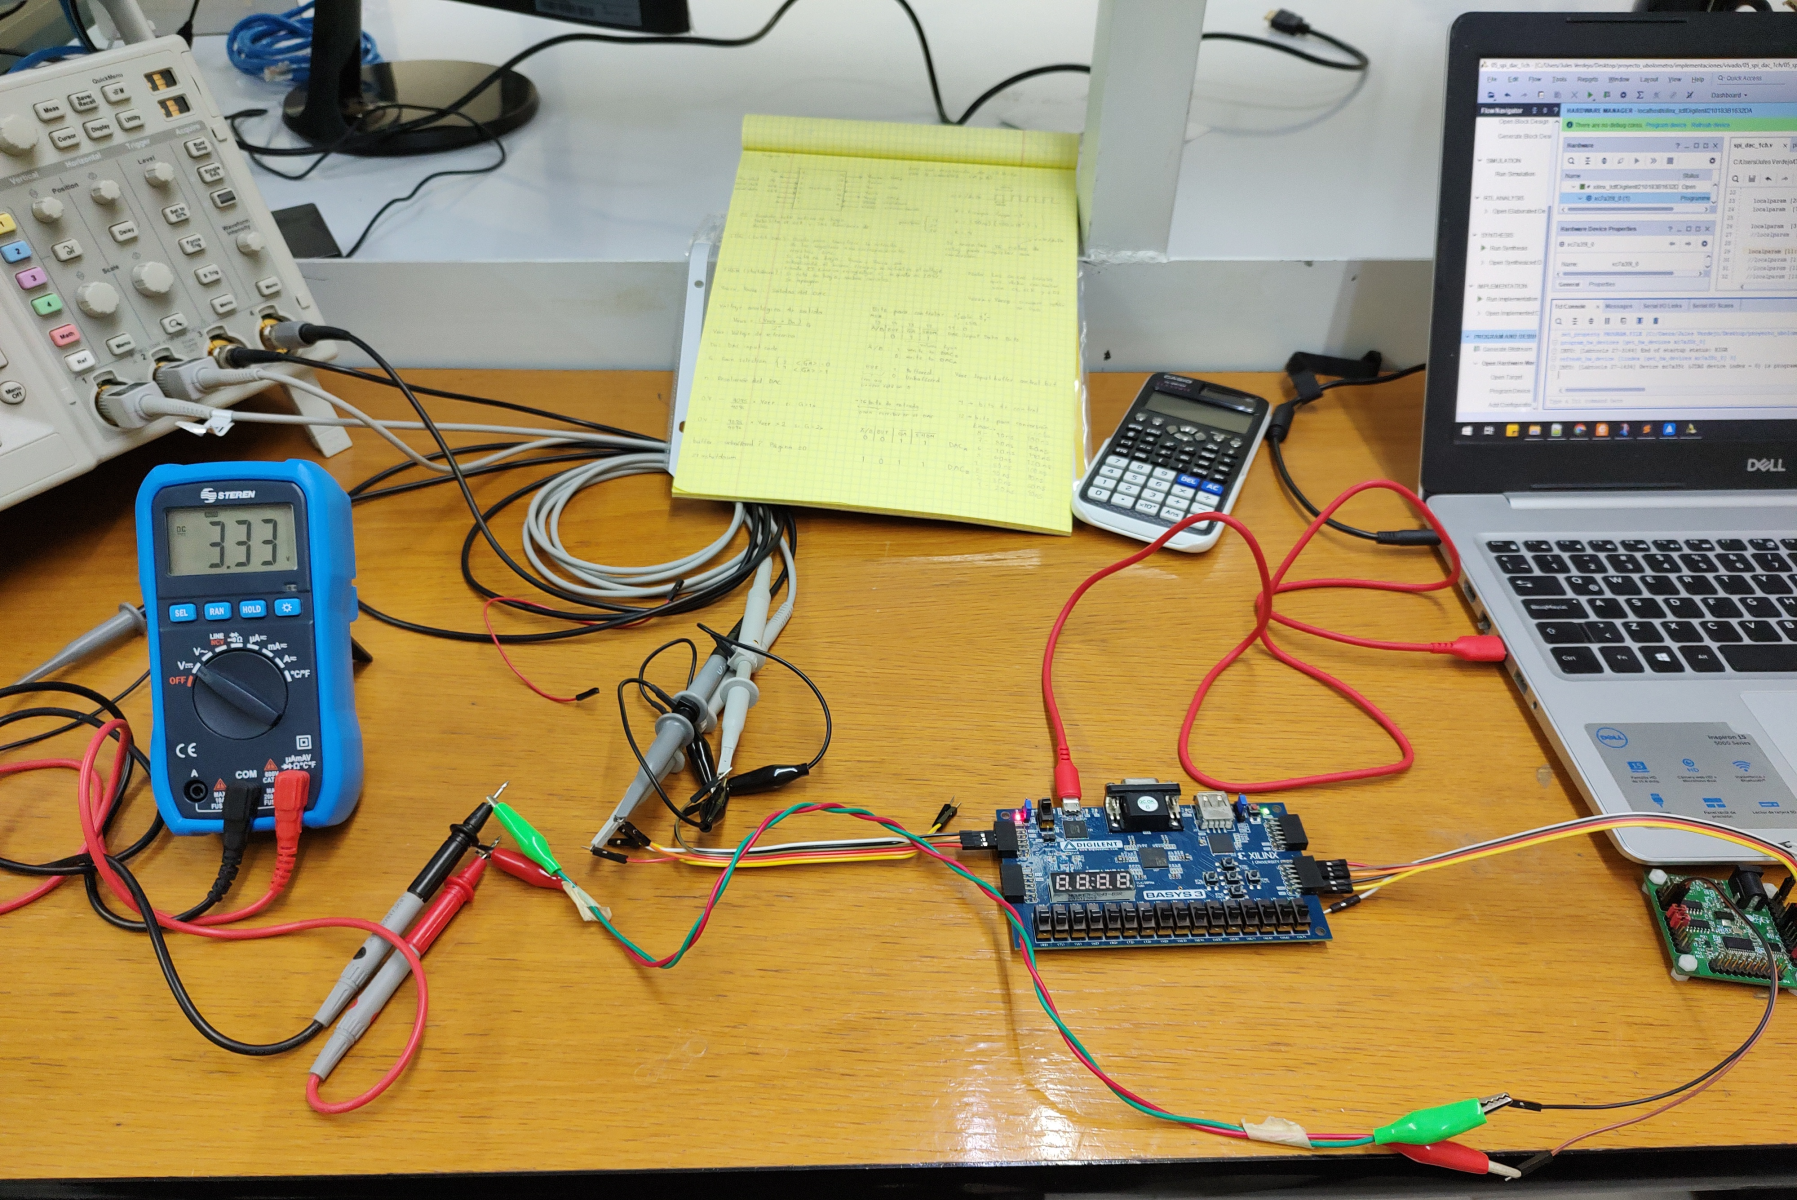
\includegraphics[width=0.6\textwidth]{dac_conversion_3v}
                \caption{Resultado de la conversión de 3.3V realizada por el DAC.}
                \label{fig:dac_conversion_3v}
            \end{figure} 
                                 
\section{Resultados de caracterización de resistencias y multiplexores}  
En esta sección se presentan los resultados combinados de la caracterización de las resistencias y de los multiplexores.


Para la caracterización de las resistencias, cada una de las $R_{test}$ seleccionadas se colocó junto con la resistencia $R_{ref}$ en un protoboard. A través de un código en MATLAB, se adquirieron 10 veces los valores de las caídas de voltaje en $R_{ref}$ correspondientes a cada uno de los voltajes de polarización, posteriormente estos fueron promediados.


En la siguiente imagen se muestra el arreglo descrito.

            \begin{figure}[hbtp]
                \centering
                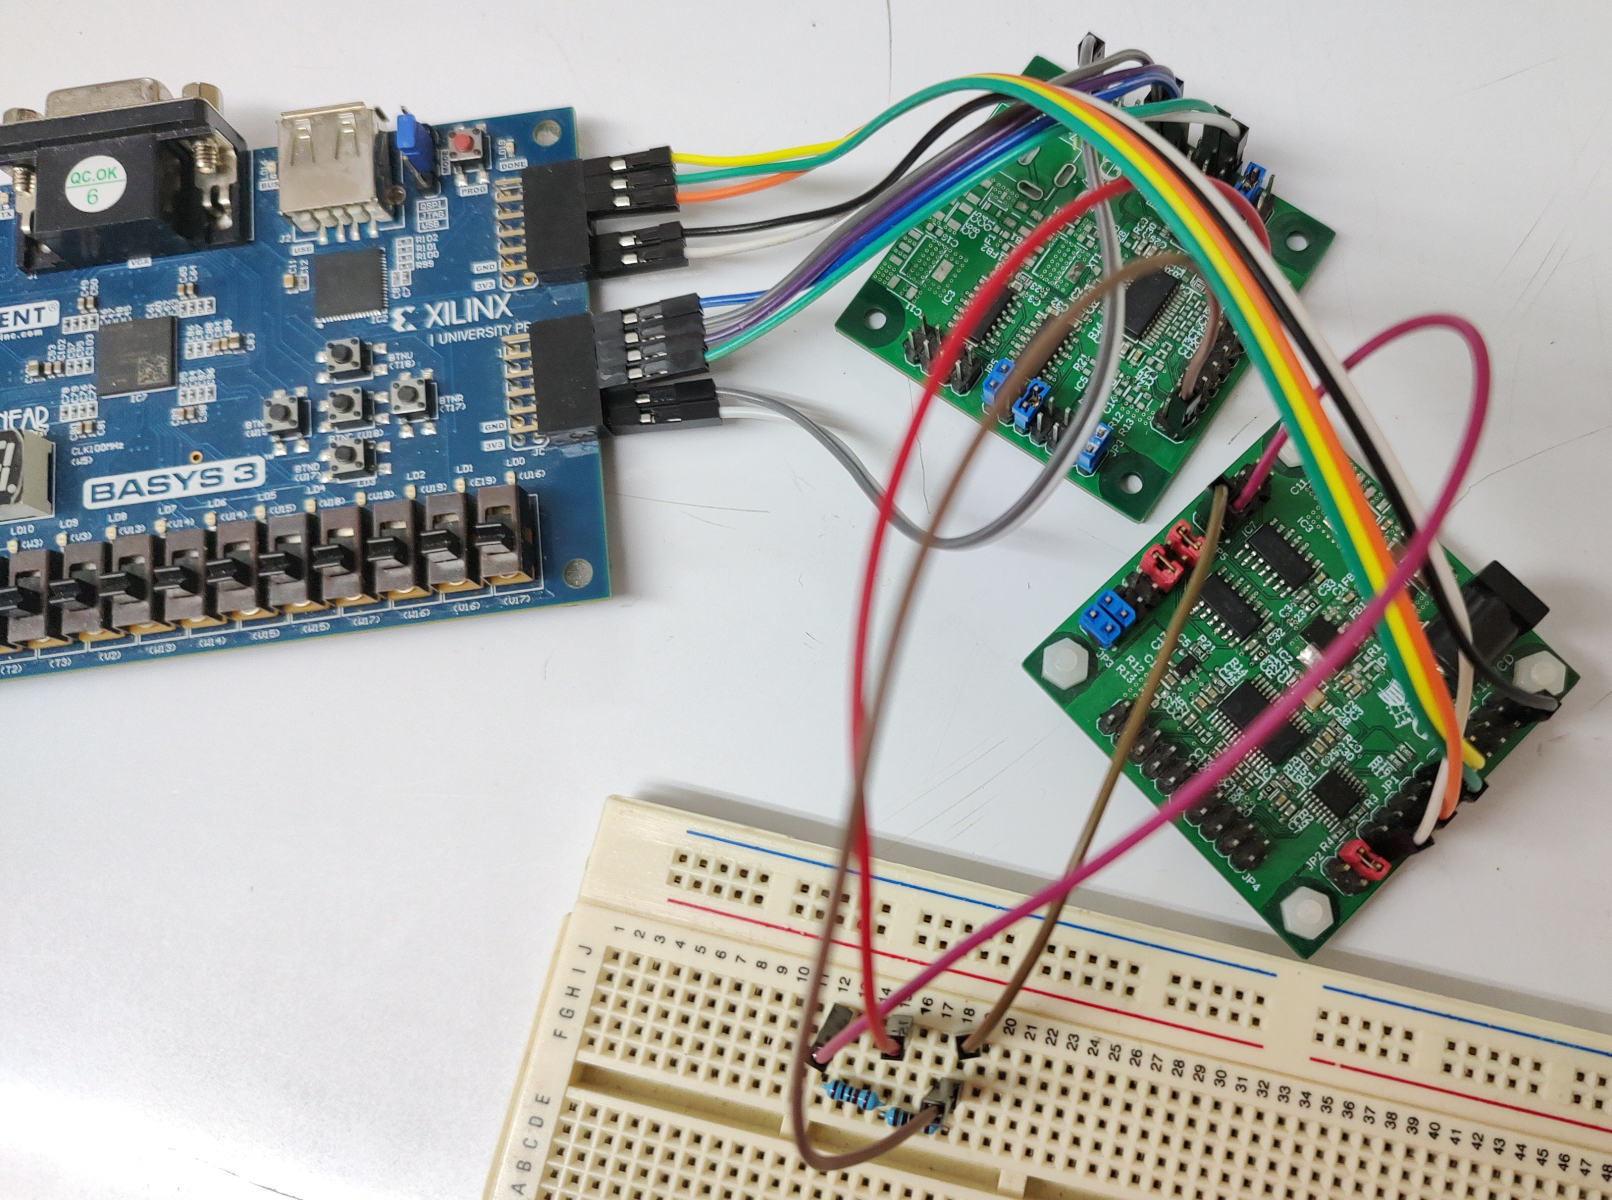
\includegraphics[width=0.6\textwidth]{divisor_proto}
                \caption{Arreglo de elementos para la caracterización de una resistencia.}
                \label{fig:divisor_proto}
            \end{figure} 

Para la caracterización de los multiplexores, se colocaron las cuatro $R_{test}$ en forma de matriz en el protoboard, la resistencia de $1K\Omega$ se ubicó en la posición (1,1), la de $3.3K\Omega$ en la (1,2), la de $5.6K\Omega$ en la (2,1) y la de $10K\Omega$ en la (2,2). Los multiplexores se conectaron para controlar tanto las filas como las columnas de la matriz, y fueron operados de manera manual. La adquisición de los valores de las caídas de voltaje se realizó de manera idéntica a la utilizada en la caracterización de una resistencia, asegurando consistencia en el proceso de medición.


El arreglo de la matriz de resistencias y multiplexores se muestra en la siguiente imagen.

            \begin{figure}[hbtp]
                \centering
                \includegraphics[width=0.6\textwidth]{matriz_resistencia}
                \caption{Arreglo de elementos para la caracterización de multiplexores.}
                \label{fig:matriz_resistencia}
            \end{figure} 

En las siguientes figuras se presentan las comparaciones de las curvas de los voltajes teóricos con los voltajes recibidos en MATLAB para cada una de las $R_{test}$, tanto con como sin multiplexores. Es notable que los multiplexores influyen en el resultado final debido a su resistencia interna, ya que cuando no se utilizan, el voltaje teórico y el voltaje recibido son muy similares. Para analizar con mayor detalle el efecto de los multiplexores, nos enfocaremos en los resultados obtenidos al polarizar el circuito con un voltaje de 3V.

            \begin{figure}[hbtp]
                \centering
                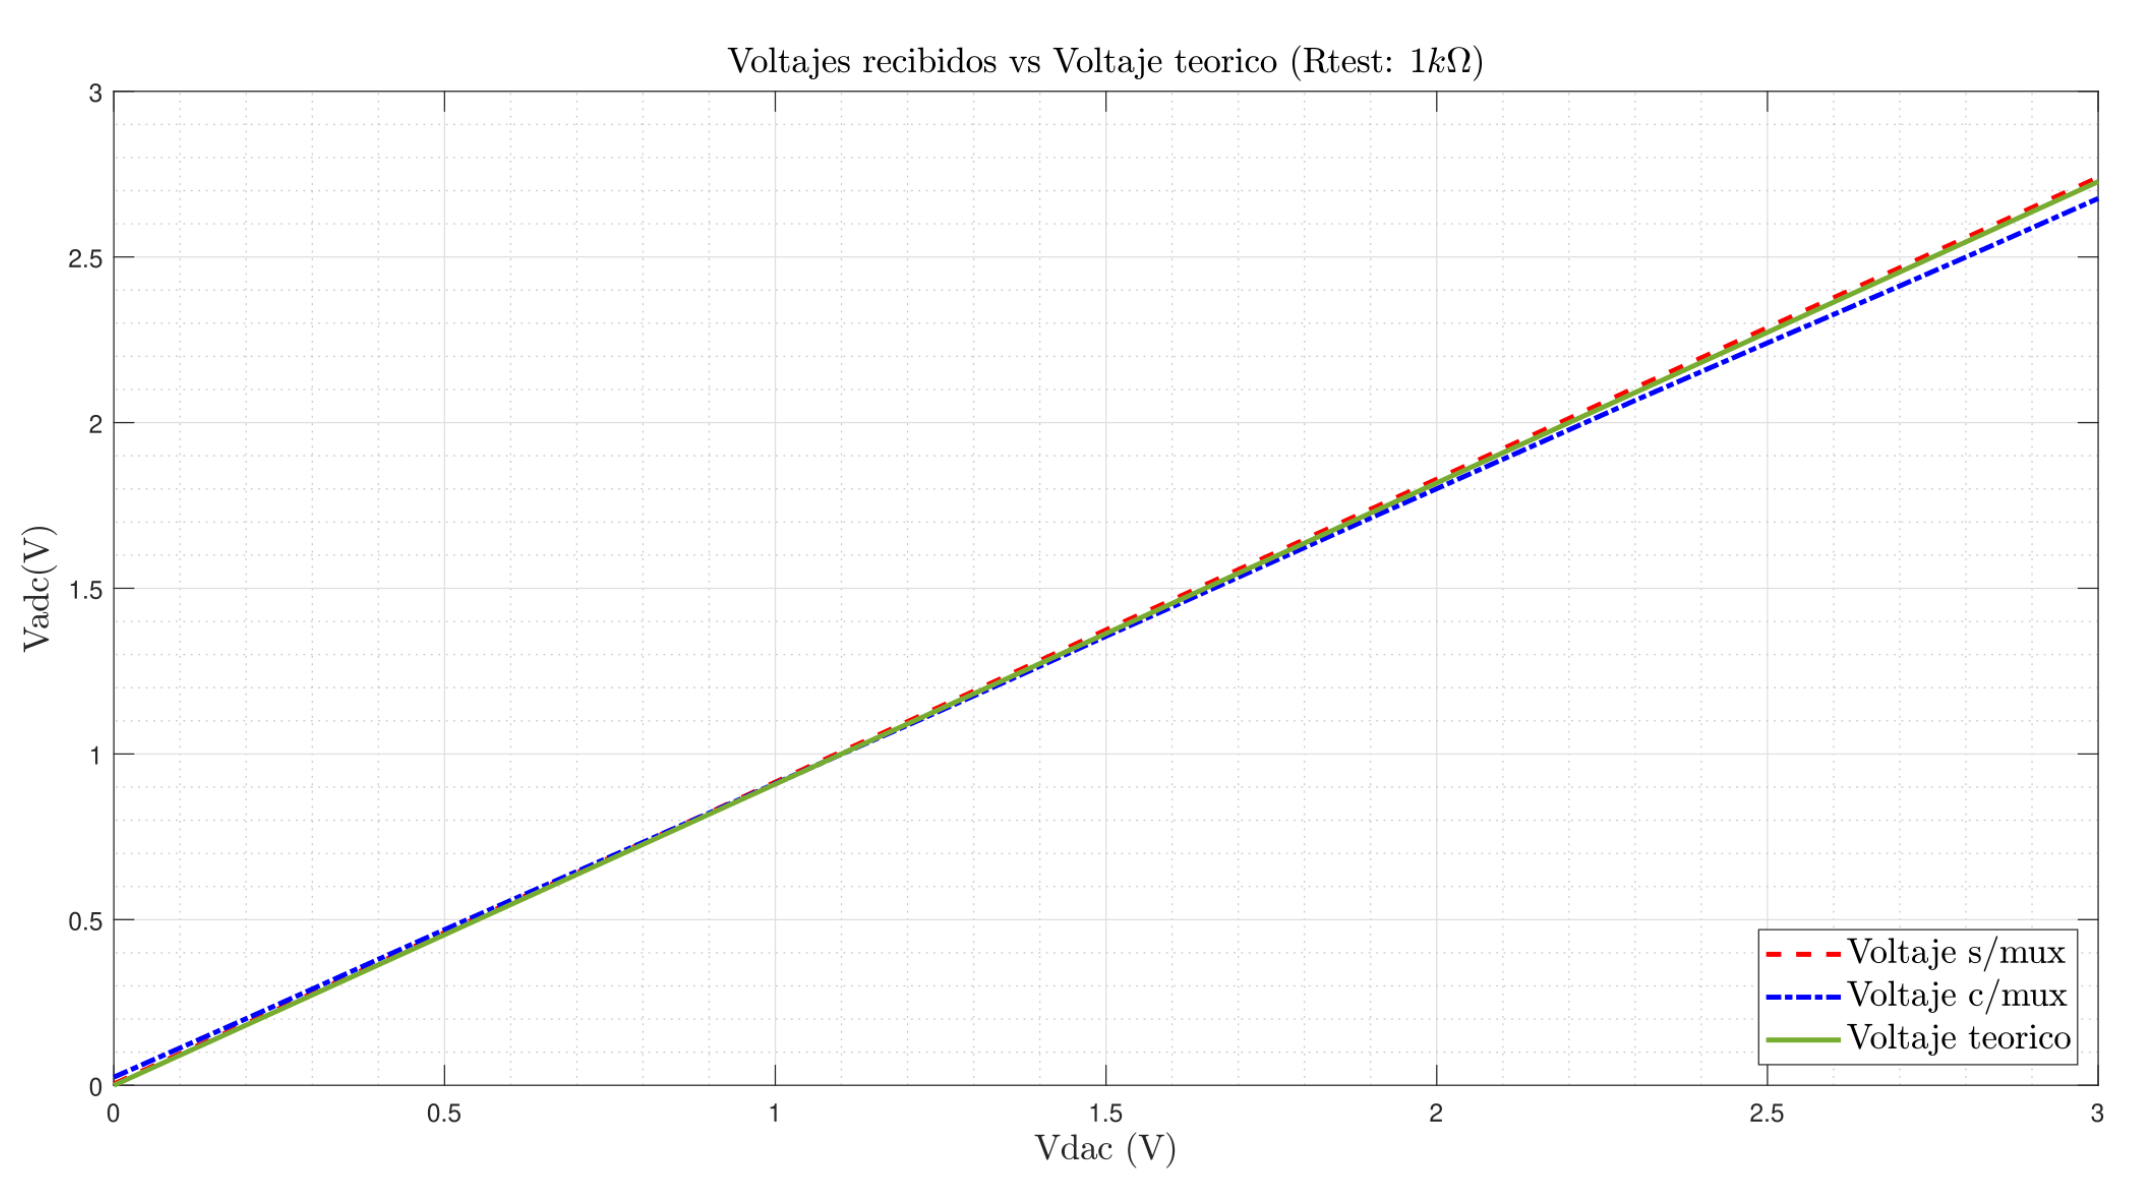
\includegraphics[width=0.9\textwidth]{01_1k}
                \caption{Voltajes teóricos vs Voltajes recibidos para $R_{test} = 1K\Omega$.}
                \label{fig:01_1k}
            \end{figure}  
\newpage
En la imagen anterior, el voltaje teórico y el voltaje recibido sin multiplexor es de 2.72V, mientras que el voltaje agregando los multiplexores también es de 2.6952V.


Para una resistencia de $3.3K\Omega$, se tiene que el valor de los voltajes teórico y sin multiplexores es de 2.2556V, y el voltaje con multiplexor igual a 2.2375V.
            
            \begin{figure}[hbtp]
                \centering
                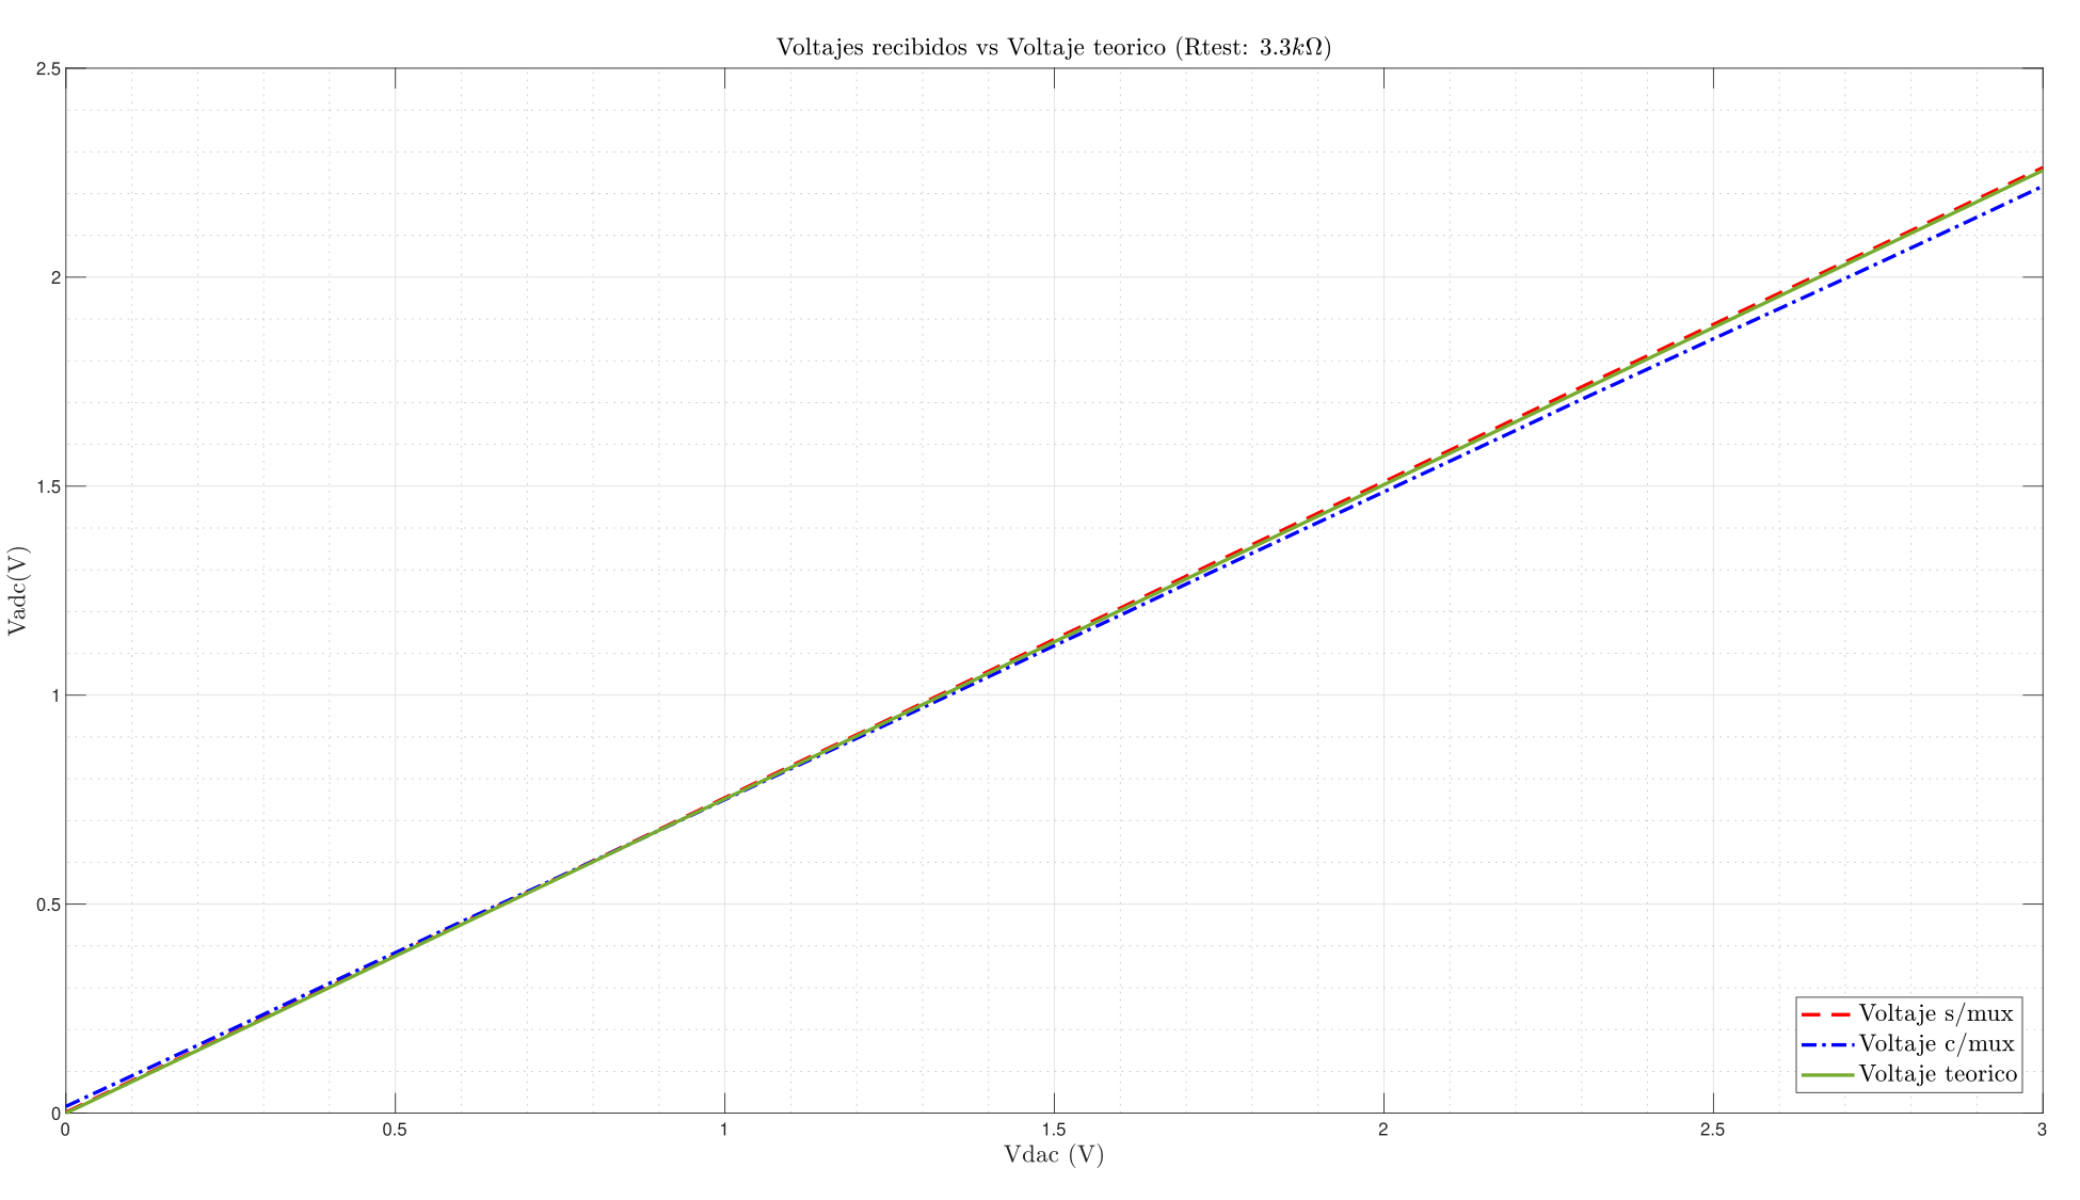
\includegraphics[width=0.9\textwidth]{02_3k3_new}
                \caption{Voltajes teóricos vs Voltajes recibidos para $R_{test} = 3.3K\Omega$.}
                \label{fig:02_3k3_new}
            \end{figure}              

Se tiene que los voltajes teórico y el de una resistencia de $5.6K\Omega$ es 1.92V, cuando se conectan los multiplexores, se registró un voltaje de 1.90V.
 
            \begin{figure}[hbtp]
                \centering
                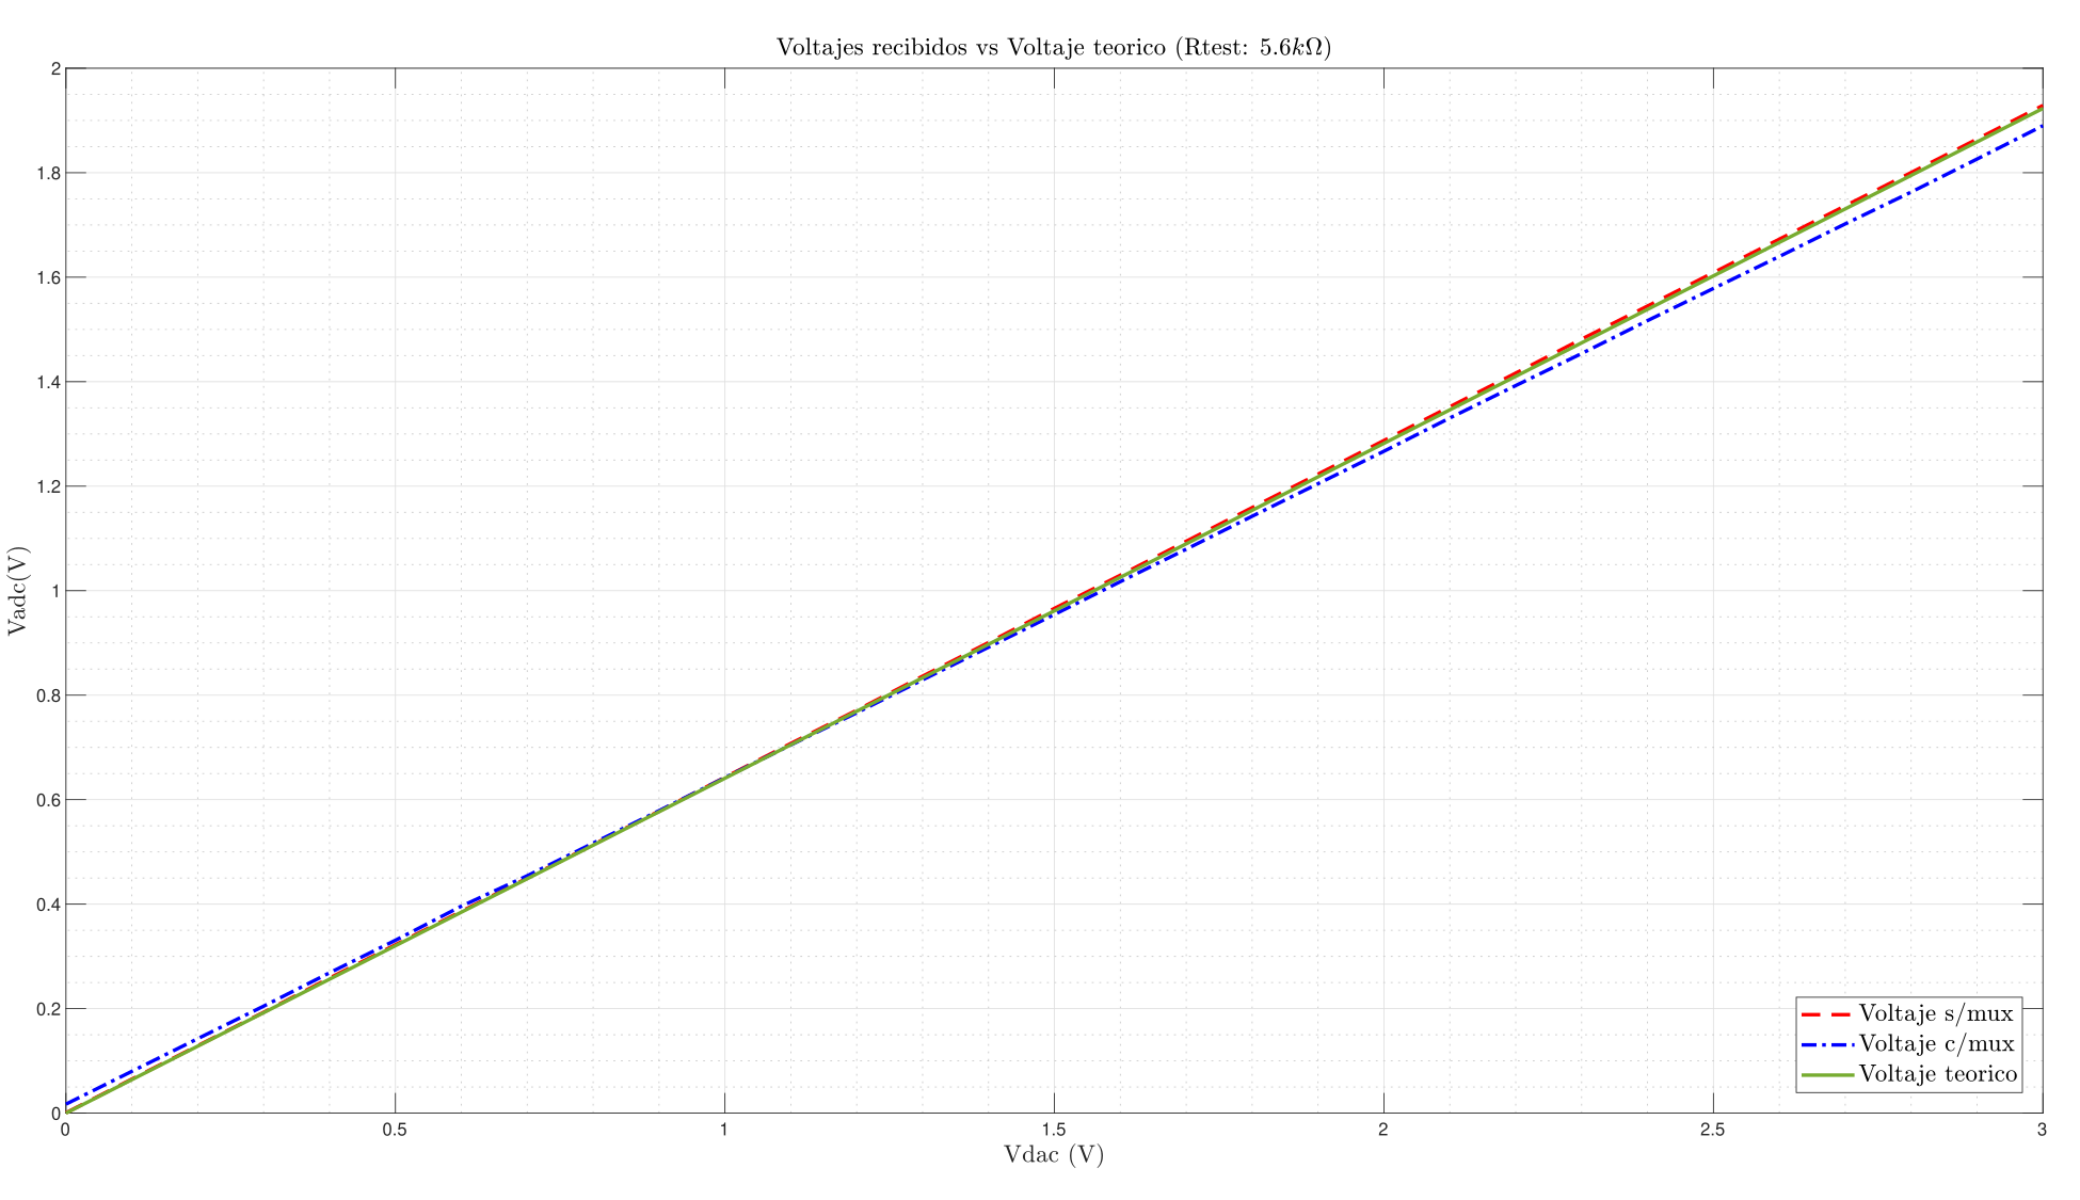
\includegraphics[width=0.9\textwidth]{03_5k6_new}
                \caption{Voltajes teóricos vs Voltajes recibidos para $R_{test} = 5.6K\Omega$.}
                \label{fig:03_5k6_new}
            \end{figure}   
\newpage
Finalmente, para una resistencia de $10K\Omega$, el voltaje teórico y el voltaje recibido es de 1.5V, y el voltaje con multiplexor de 1.49V.

            \begin{figure}[hbtp]
                \centering
                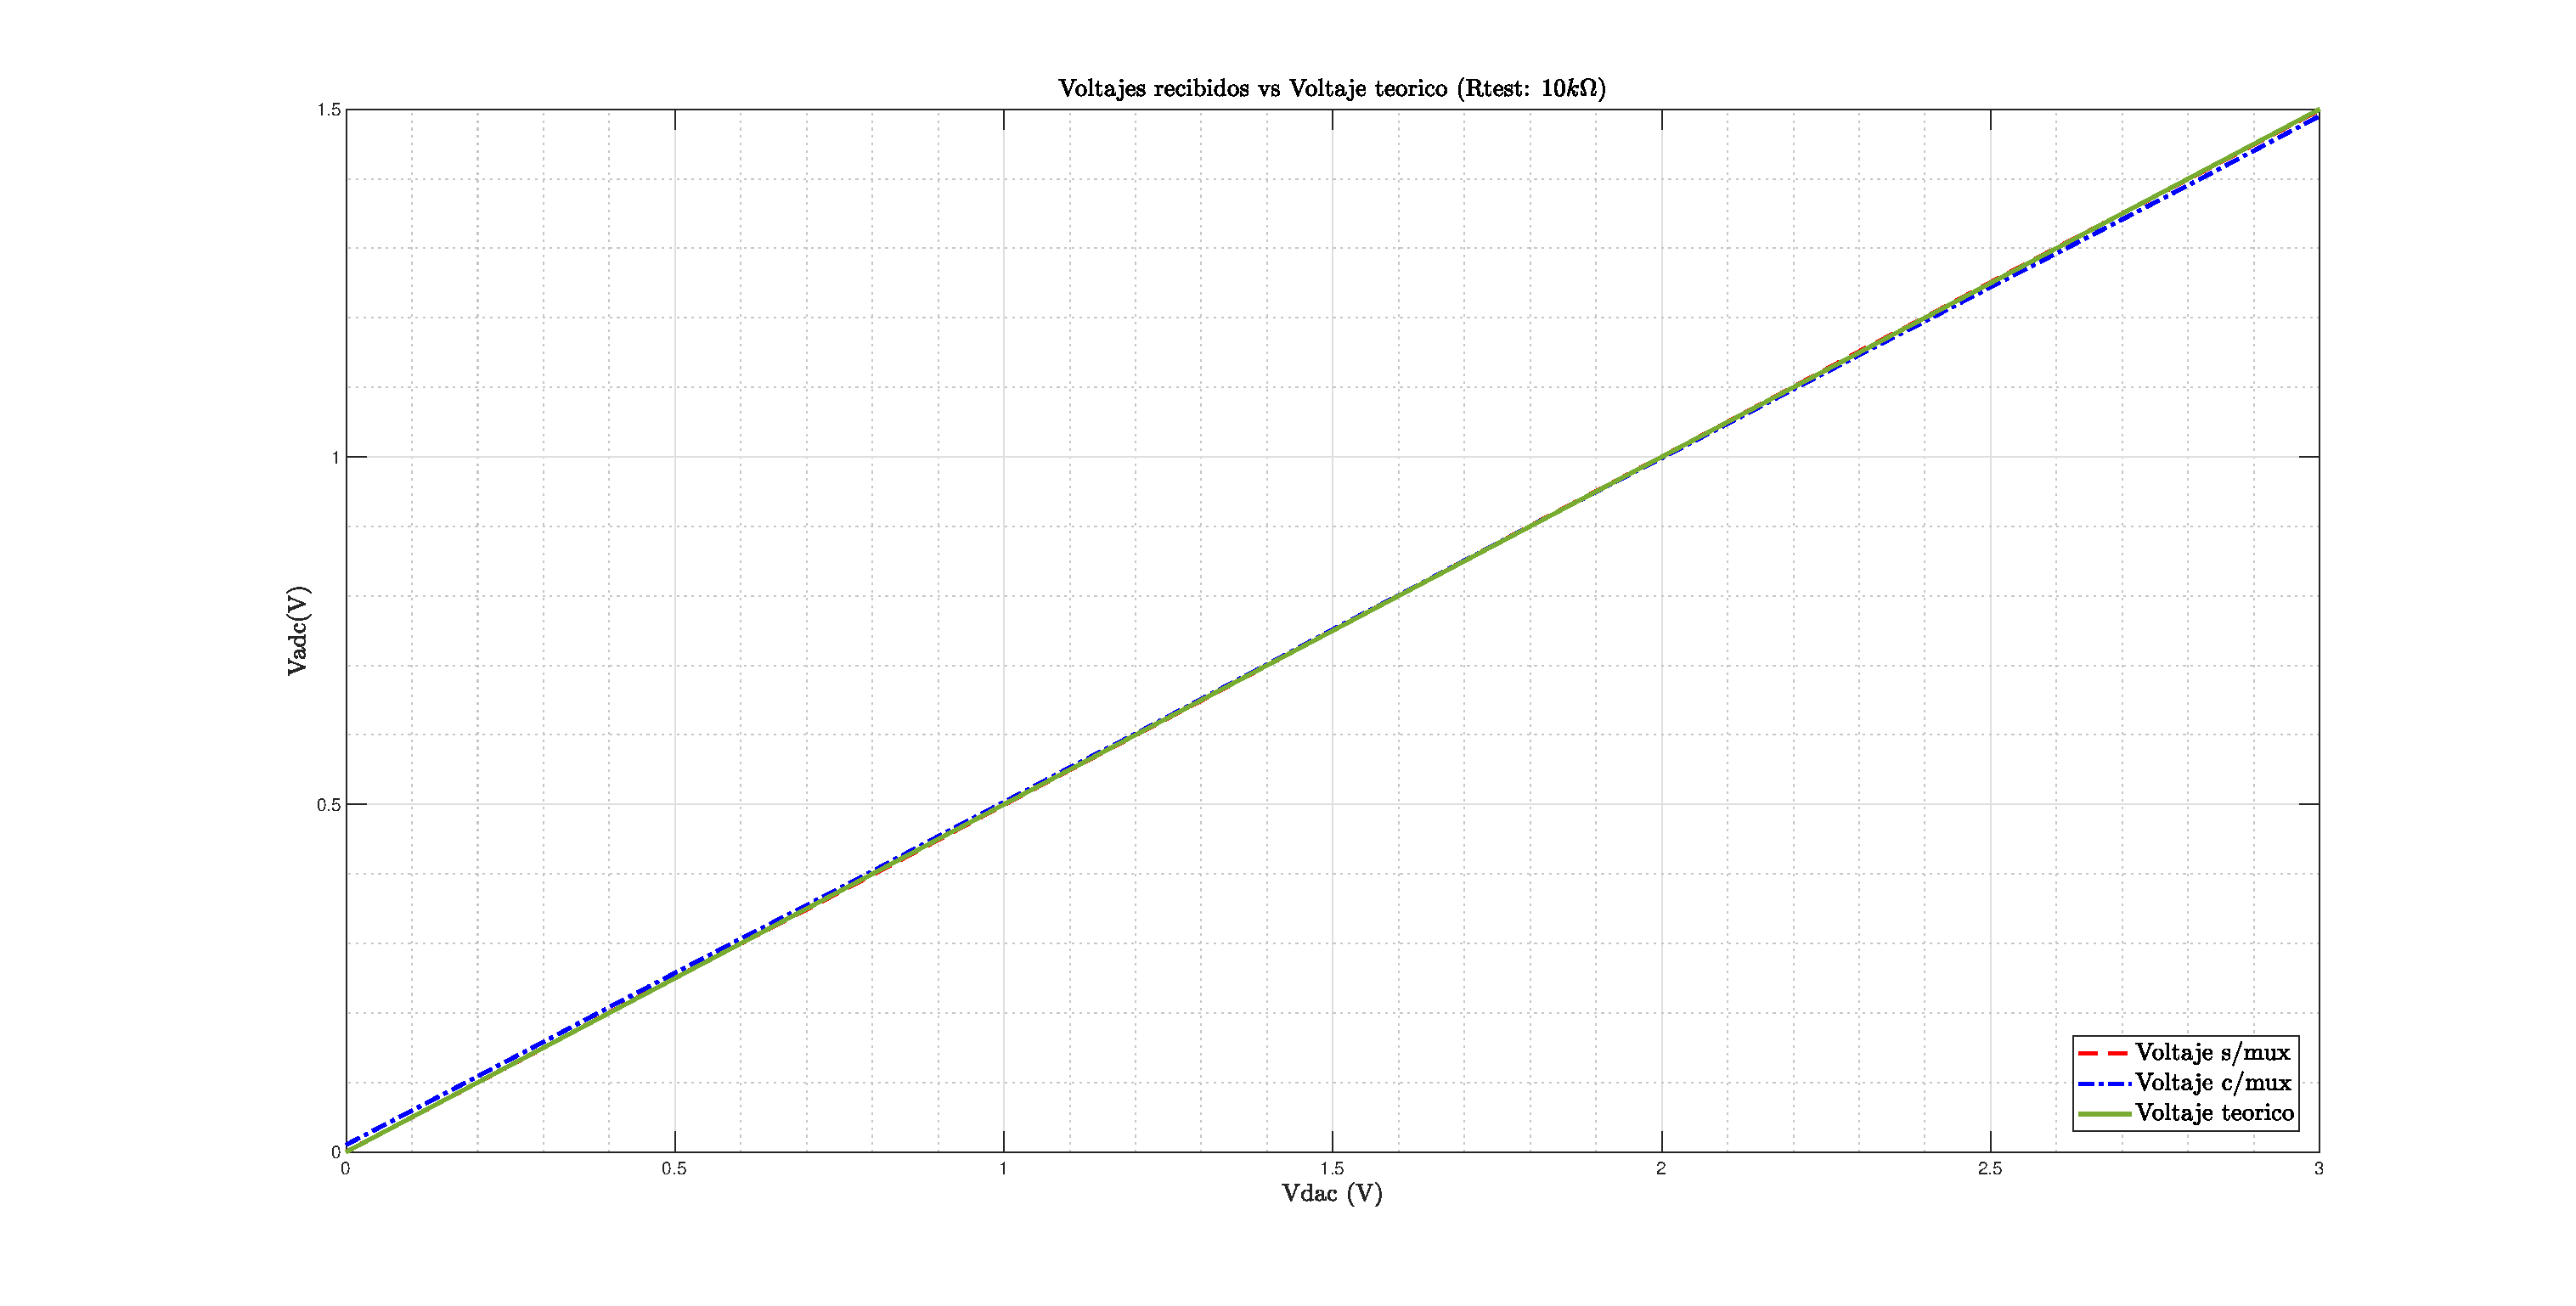
\includegraphics[width=0.9\textwidth]{04_10k_new}
                \caption{Voltajes teóricos vs Voltajes recibidos para $R_{test} = 10K\Omega$.}
                \label{fig:04_10k_new}
            \end{figure}  

La resistencia interna de los multiplexores, fue medida con un multímetro, manteniendo el voltaje de polarización del circuito fijo en 3V. En la siguiente tabla se muestran los valores obtenidos de las resistencias internas de los multiplexores.

               
            \begin{table}[htbp]
                \caption{Resistencia de multiplexores.}
                \begin{center}
                    \resizebox{0.9\linewidth}{!}{ 
                    \begin{NiceTabular}{| c | c | c | c | c | c |}
                        \CodeBefore
                        \Body
                        \hline
                        \textbf{$R_{test}$}  & \textbf{$V_{muxrows}$} & \textbf{$V_{muxcols}$} & \textbf{$i$} & \textbf{$R_{mux_{row}}$} & \textbf{$R_{mux_{col}}$}\\
                        \hline
                        1K$\Omega$   & 3.86e-2 V& 3.5e-2  V& 2.65e-4 A& 145.66 $\Omega$& 132$\Omega$\\
                        3.3K$\Omega$ & 3.43e-2 V& 3.1e-2  V& 2.21e-4 A& 155.2 $\Omega$& 140.27$\Omega$\\
                        5.6K$\Omega$ & 2.83e-2 V& 2.48e-2 V& 1.89e-4 A& 149.73 $\Omega$& 131.21$\Omega$\\
                        10K$\Omega$  & 2.25e-2 V& 2.11e-2 V& 1.49e-4 A& 151 $\Omega$& 141.6$\Omega$\\                            
                        \hline
                    \end{NiceTabular}
                    }
                \label{tab:Mux_res}
                \end{center}
            \end{table}

De acuerdo con el datasheet, las resistencias de cada una de las entradas/salidas Yn varían. Según los datos presentados en la tabla, la resistencia interna de los multiplexores se encuentra en un rango de 130 a 160 $\Omega$. 
 
                     
\section{Resultados de caracterización de fotorresistencia}
Para caracterizar la fotorresistencia, inicialmente se expuso a la iluminación de una lámpara de un salón, pero el valor de la resistencia no lograba estabilizarse. Posteriormente, se intentó medir la fotoresistencia en oscuridad, pero esta superaba los $5M\Omega$, lo que impedía que el multímetro detectara su valor y que esta pudiera ser caracterizada, debido a que, al ser una resistencia muy grande, la caída de voltaje en el circuito de lectura sería tan pequeña que el ADC no podría convertir. Por lo tanto, se optó por colocar la fotorresistencia en condiciones ideales y controladas, dentro de una caja oscura, y variando la intensidad de un LED de 3W mediante un PWM con distintos duty cycles. De esta forma, se obtuvieron valores de resistencia adecuados para su caracterización.

            \begin{figure}[hbtp]
                \centering
                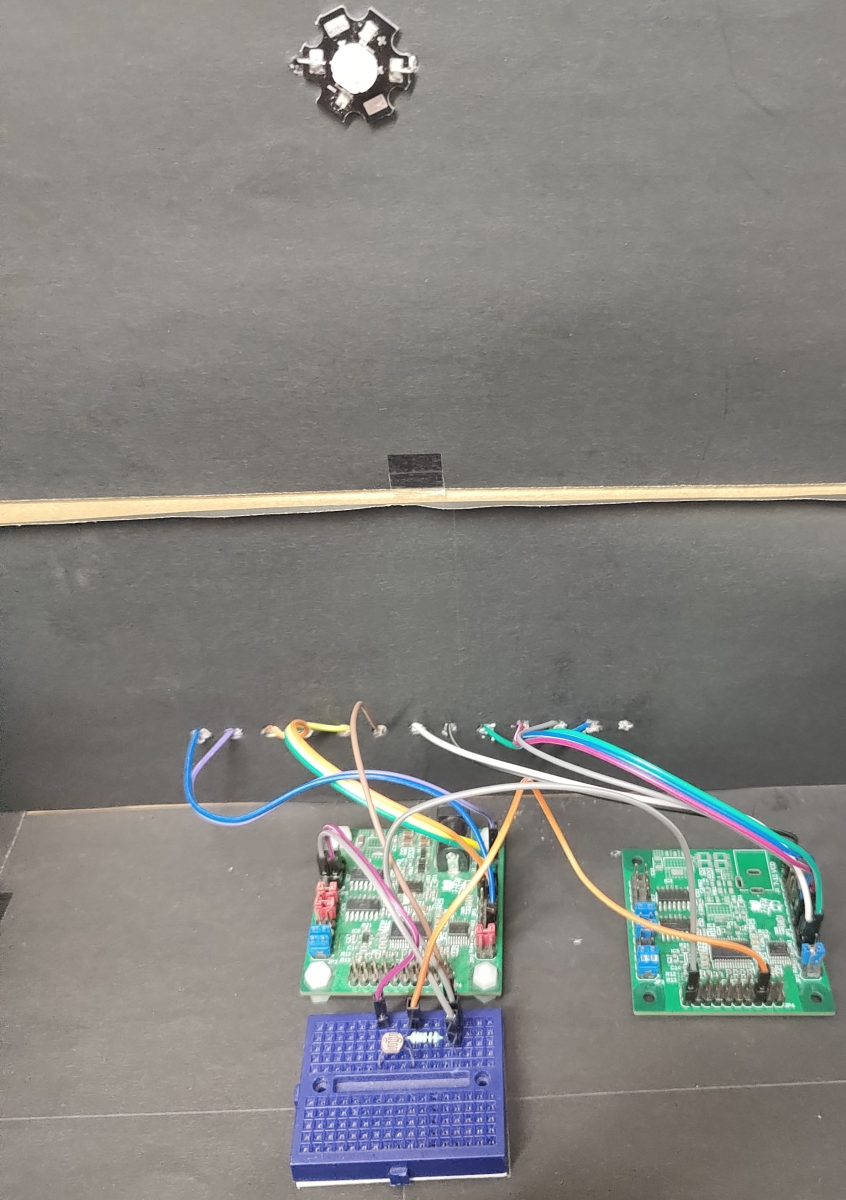
\includegraphics[width=0.4\textwidth]{fotores_box}
                \caption{Arreglo de fotoresistencia para su caracterización.}
                \label{fig:fotores_box}
            \end{figure}

Antes de caracterizar la fotorresistencia bajo condiciones ideales, fue necesario definir el voltaje adecuado para alimentar el LED de 3W, ya que el brillo del LED varía en función del voltaje aplicado. Inicialmente, el LED se alimentó con 3V, variando el duty cycle del PWM y midiendo la resistencia de la fotorresistencia en cada caso. Posteriormente, el proceso se repitió alimentando el LED con 3.3V y, finalmente, con 3.5V. Estas mediciones permitieron observar cómo el voltaje de alimentación del LED influye en la respuesta de la fotorresistencia.


En la siguiente tabla se muestran los valores de la fotorresistencias bajo distintos voltajes de polarización y duty cycles.
\newpage
            \begin{table}[htbp]
                \caption{Valor de fotorresistencias con diferentes duty cycles.}
                \begin{center}
                    \resizebox{0.5\linewidth}{!}{ 
                    \begin{NiceTabular}{| c | c | c |}
                        \CodeBefore
                        \Body
                        \hline
                        \textbf{$V_{Fuente}$}  & \textbf{Duty cycle ($\%$)} & \textbf{$R_{med} (K\Omega)$} \\
                        \hline
                        3 V     & 25  & 210 - 213.7\\
                                & 50  & 104 - 105.7\\
                                & 75  & 70 -71\\
                                & 100 & 53 - 54\\ \hline
                        3.3 V   & 25  & 24 - 31\\
                                & 50  & 15 - 18\\
                                & 75  & 10 - 12\\
                                & 100 & 8 - 9\\ \hline
                        3.5 V   & 25  & 6 - 7\\
                                & 50  & 3.6\\
                                & 75  & 2.6\\
                                & 100 & 2\\                             
                        \hline
                    \end{NiceTabular}
                    }
                \label{tab:Duty_cycle}
                \end{center}
            \end{table}

Dado que con un voltaje de polarización de 3.3V se obtuvieron valores de resistencia más adecuados para la caracterización de la fotorresistencia, y que esta presentó diferentes valores a distintos duty cycles, se optó por alimentar el LED con ese voltaje. Esto permitió una mejor evaluación del comportamiento de la fotorresistencia bajo condiciones controladas de iluminación.


El circuito de lectura utilizado para la caracterización de la fotorresistencia fue nuevamente una resistencia de $10K\Omega$. El diseño digital empleado para esta caracterización es el mismo que se utilizó en las etapas anteriores.


En la siguiente imagen se muestran las curvas de voltaje de la fotorresistencia a diferentes duty cycles. 
%\newpage            
            \begin{figure}[hbtp]
                \centering
                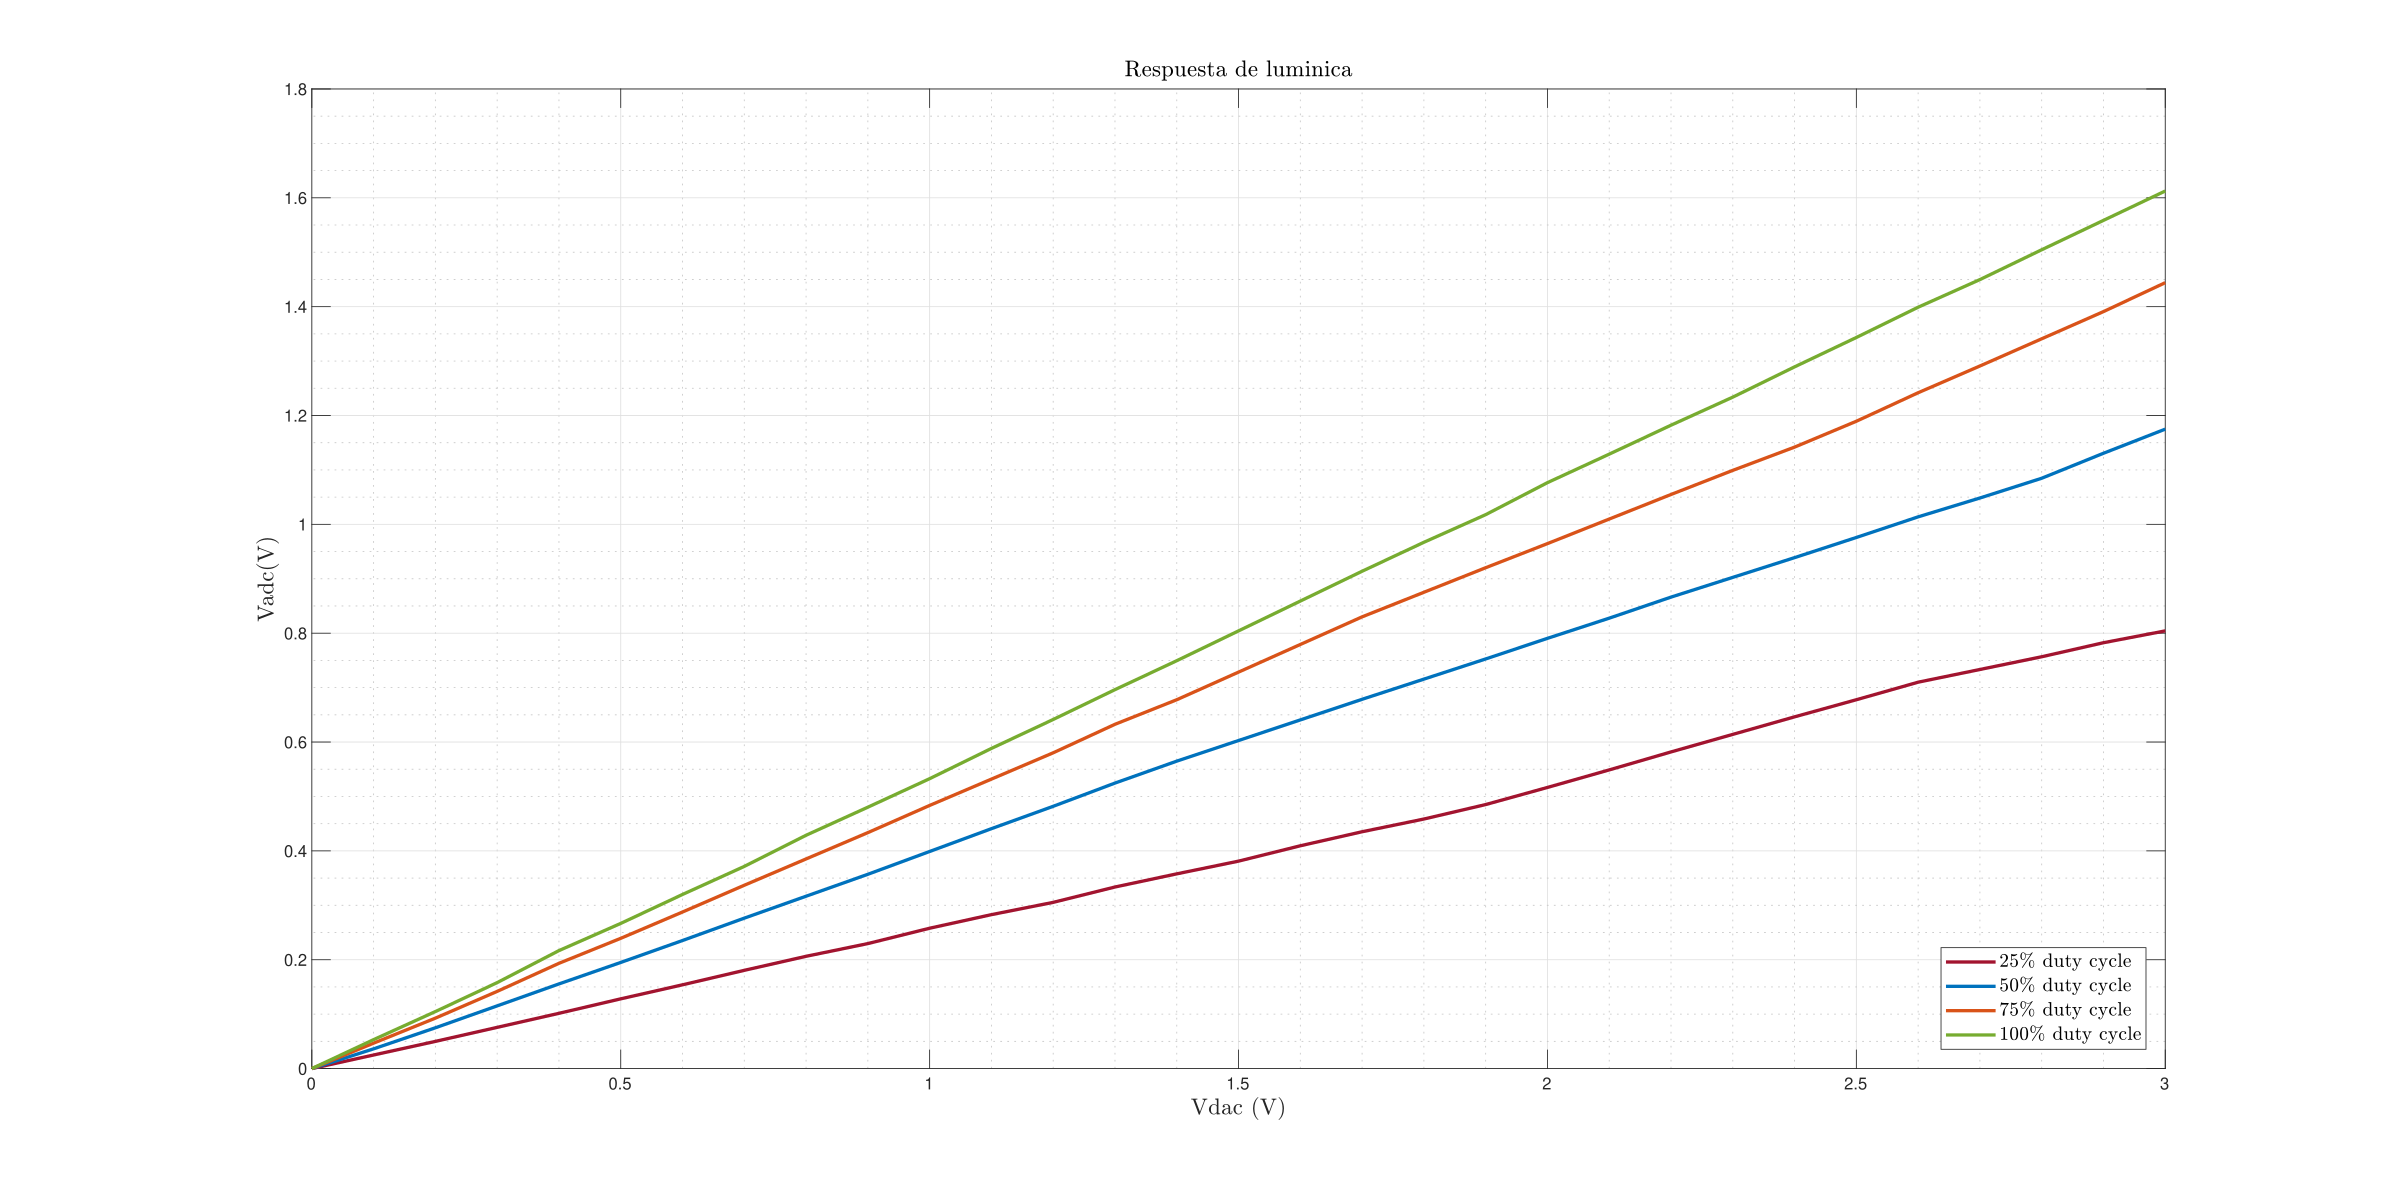
\includegraphics[width=1\textwidth]{respuesta_luminica}
                \caption{Respuesta lumínica.}
                \label{fig:respuesta_luminica}
            \end{figure}            
            
Usando la ecuación del divisor de voltaje, se determinó que los valores obtenidos de la fotorresistencia coinciden con los presentados en la Tabla \ref{tab:Duty_cycle}. Además, en la imagen se puede observar que, a mayor iluminación, la fotorresistencia presenta un comportamiento más lineal.            

\section{Resultados de las imágenes obtenidas}
De acuerdo al datasheet de la fotorresistencia, su tiempo de respuesta es de 20 ms después de haber sido expuesta a la luz durante 2 horas. Debido a este comportamiento, no se pudo generar una imagen con estos elementos, ya que el tiempo necesario para obtenerla sería demasiado extenso. Por este motivo, se optó por utilizar fototransistores, que ofrecen un tiempo de respuesta mucho más rápido y adecuado para la captura de imágenes en menos tiempo.


Para obtener imágenes utilizando la matriz de 8x8 fototransistores, se propusieron las máscaras mostradas en la Figura \ref{fig:mask_final}.
            \begin{figure}[hbtp]
                \centering
                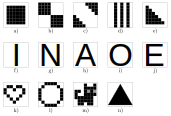
\includegraphics[width=0.8\textwidth]{mask_final}
                \caption{Máscaras propuestas.}
                \label{fig:mask_final}
            \end{figure}  

Cada una de estas máscaras fue colocada encima de la matriz, que fue iluminada con el LED de un celular situado a 20 cm de distancia. Las variaciones de voltaje del circuito de lectura fueron adquiridas y procesadas en MATLAB.

            \begin{figure}[hbtp]
                \centering
                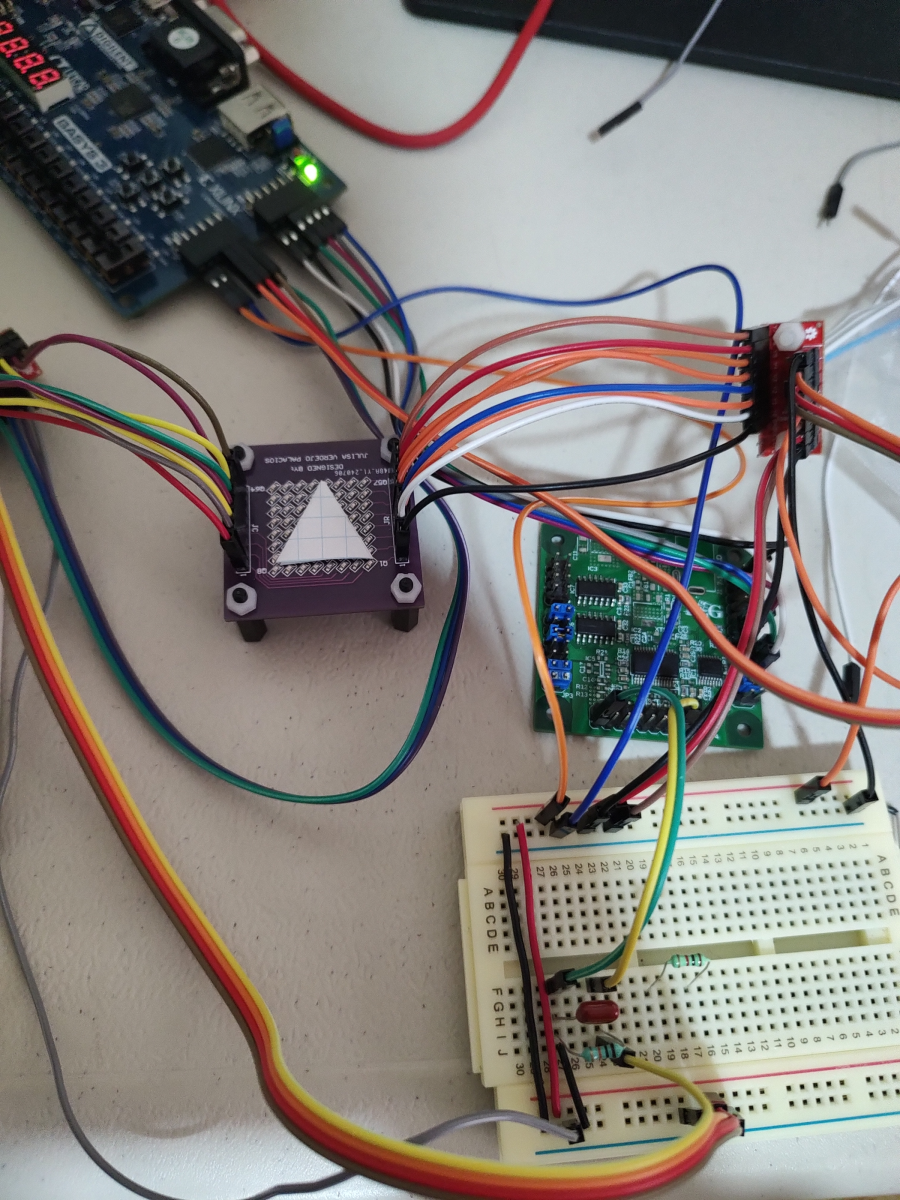
\includegraphics[width=0.4\textwidth]{matrix_mask}
                \caption{Máscara triangular colocada encima de la matriz de fototransistores.}
                \label{fig:matrix_mask}
            \end{figure} 
\newpage
En la Figura \ref{fig:result_mask} se muestran las imágenes obtenidas al colocar cada una de las máscaras sobre la matriz de 8$\times$8 fototransistores. 


El diseño del sistema de adquisición de datos y la PCB funcionaron con éxito, permitiendo generar imágenes que son muy similares a las formas de las máscaras utilizadas. Esto demuestra la efectividad del sistema para capturar y reproducir las variaciones de luz.


            \begin{figure}[hbtp]
                \centering
                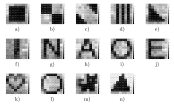
\includegraphics[width=0.8\textwidth]{result_mask}
                \caption{Resultados de las máscaras aplicadas a los fototransistores.}
                \label{fig:result_mask}
            \end{figure}
